\documentclass{ximera}

\newcommand{\RR}{\mathbb R}
\renewcommand{\d}{\,d}
\newcommand{\dd}[2][]{\frac{d #1}{d #2}}
\renewcommand{\l}{\ell}
\newcommand{\ddx}{\frac{d}{dx}}
\newcommand{\dfn}{\textbf}
\newcommand{\eval}[1]{\bigg[ #1 \bigg]}

\title{Precalculus Review - Section 1}

\begin{document}
\begin{abstract}
%
\end{abstract}
\maketitle

This section contains review material on:
\begin{itemize}
	\item Real numbers, intervals, and absolute values
	\item Radical and rational expressions
	\item Polynomials
	\item Fractional expressions
\end{itemize}

\section{Real Numbers and its Famous Subsets}
In Calculus, we deal with the set of real numbers and its subsets.  One important subset is the set of \emph{integers}
\[ \ldots, -3, -2, -1, 0, 1, 2, 3, 4, \ldots \]

The numbers $0, 1, 2, 3, 4, \ldots$ are called the \emph{non-negative integers}; the set of \emph{natural numbers} consists of
the numbers $1, 2, 3, 4, \ldots$.  The quotient $\displaystyle \frac{p}{q}$ of two integers $p$ and $q$ (where $q \neq 0$) is called
a \emph{rational number}.  For example, $\frac{1}{3}$, $-\frac{4}{11}$, $0.47=\frac{47}{100}$,
$-32 = \frac{-32}{1}$, and $13 = \frac{13}{1}$ are all rational numbers.  (Looking at the last two examples,
we see that integers belong to the set of rational numbers.)  It is important to remember that division by zero is not allowed.  Expressions such as $\frac{7}{0}$ or $\displaystyle \frac{0}{0}$ are not defined.  However, zero divided by a non-zero number is zero; for example $\frac{0}{7} = 0$ and $\displaystyle \frac{0}{-11}=0$.

The numbers that cannot be represented as quotients of rational numbers are called \emph{irrational numbers}.  Numbers such as $\sqrt{2}$, $\pi$, $\sqrt{5}$, and $\log_{10} 2$ are irrational.  The set of real numbers consists of the rational and irrational numbers.  It is usually denoted by $\RR$. We can use decimal notation to express real numbers.  Rational numbers have a repeating decimal representation; for example, $\frac{1}{2}=0.50000000=0.5\bar{0}$, $\frac{1}{3}=0.33333=0.\bar{3}$, $\frac{13}{44}=0.295454545 = 0.29\bar{54}$, etc. Non-repeating decimal expressions represent irrational numbers: $\pi = 3.1415926535\ldots$, $\sqrt{2}=1.414213562\ldots$, etc.

\subsection*{Real Numbers are Ordered}
$a < b$ means that ``$a$ is less than $b$'', $a > b$ means that ``$a$ is greater than $b$'', $a \leq b$ means that ``$a$ is less than $b$ or $a$ is equal to $b$'', and $a \geq b$ means that ``$a$ is greater than $b$ or $a$ is equal to $b$.''  For example, $\sqrt{2} < 1.42$, $\displaystyle \frac{3}{5} \geq 0.6$, $4 \leq 4$, $\pi > 3.1415$, etc.

\subsection*{Number Line and Intervals}
The Real numbers can be represented visually as points on a number line, see the figure below.

\begin{image}
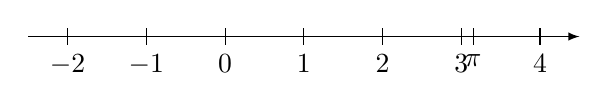
\begin{tikzpicture}
	\draw[-latex] (-2.5,0) -- (4.5,0) ;
	\foreach \x in  {-2,-1,0,1,2,3,4}
		\draw[shift={(\x,0)},color=black] (0pt,3pt) -- (0pt,-3pt);
	\foreach \x in {-2,-1,0,1,2,3,4}
		\draw[shift={(\x,0)},color=black] (0pt,0pt) -- (0pt,-3pt) node[below]{$\x$};
	\draw[shift={(3.15,0)},color=black] (0pt,3pt) -- (0pt, -3pt);
	\draw[shift={(3.15,0)},color=black] (0pt,0pt) -- (0pt, -3pt) node[below]{$\pi$};
\end{tikzpicture}
\end{image}

We chose an arbitrary point on the line to be the \emph{origin} (denoted by O, it represents the number zero), and indicate
the direction in which the numbers increase by an arrow.  For example, $a < b$ means that $a$ lies to the left of $b$ on the number line.

An \emph{open interval} $(a,b)$ consists of all real numbers between $a$ and $b$, not including $a$ and not including $b$.  In symbols, $(a,b)$
consists of all real numbers $x$ such that $a < x < b$.  If we need to include endpoints, we use square brackets. For example, $[a,b)$ represents all real
numbers $x$ such that $a \leq x < b$.  In words, the interval $[a,b)$ consists of all real numbers between $a$ and $b$, including $a$ but not including $b$.

To denote the set of all numbers that are greater than $a$, we use $(a, \infty)$.  If we need all numbers that are greater than or equal to $a$, we use
$[a,\infty)$.  The numbers smaller than $b$ form the interval $(-\infty, b)$.  Remember that $\infty$ and $-\infty$ are not real numbers (thus, when infinity is
involved, we always use round parentheses).

We could also use set-theoretic notation. For example, $[a,b) = \{ x \in \RR \, | \, a \leq x < b\}$, $(-\infty, b] = \{x \in \RR \, | \, x \leq b \}$,
or $(a, \infty) = \{ x \in \RR \, | \, x > a\}$.

\begin{example}
Describe the following sets of real numbers in interval notation:
\begin{enumerate}
	\item $\{ x \in \RR \, | \, 4 \leq x \leq 7 \} = [4,7)$
	\item All real numbers smaller than 3 $= (-\infty, 3)$
	\item $\{ x \in \RR \, | \,  x \leq -31 \} = (-\infty, -31]$
	\item All real numbers $=(-\infty, \infty)$
\end{enumerate}
\end{example}

\section{Absolute Value}
The absolute value of a real number $a$ is defined as
\[ |a| = \begin{cases} a & \textrm{ if } a \geq 0\\
                       -a & \textrm{ if } a < 0 \end{cases} \]

Thus, $|6| = 6$, $|0| = 0$, and $|-13| = -(-13) = 13$.

The distance between any two numbers $a$ and $b$ on a number line is given by $|b-a|$.

\begin{theorem}[Properties of Absolute Value]
  Suppose that $a$ and $b$ are any two real numbers. Then:
  \begin{itemize}
    \item $|ab|=|a||b|$
    \item $\left|\frac{a}{b}\right|=\frac{|a|}{|b|}$
    \item $\left|a^n\right|=|a|^n$
  \end{itemize}
\end{theorem}

\section{Integers as Exponents}
If $a$ is a real number and $n=1,2,3, \ldots$ a positive integer, then
\[ a^n = \underbrace{a \cdot a \cdot a \cdot \ldots \cdot a}_{n \textrm{ factors}} \]

By definition, $a^0 = 1$ (for $a \neq 0$).  We usually drop the exponent $1$, and write $a$ instead of $a^1$.  If $a \neq 0$ and $n = 1, 2, 3, \ldots$,
then we define \[ a^{-n} = \frac{1}{a^n}. \]

\begin{theorem}[Rules for Exponents]
Suppose that $a\neq 0$, and $m,n$ are integers. Then:
  \begin{itemize}
	  \item $a^m \cdot a^n = a^{m+n}$
    \item $(ab)^n = a^n b^n$
    \item $\left(a^m\right)^n = a^{mn}$
    \item $\frac{a^m}{a^n} = a^{m-n}$
    \item $\frac{a^n}{b^n} = \left( \frac{a}{b} \right)^n$
  \end{itemize}
\end{theorem}

\section{Radicals and Rational Exponents}
The equation $a^n = b$, $(n=2,3,4,\ldots)$ can also be written as $a=\sqrt[n]{b}$.  If $n=2$, then $\sqrt[2]{b}$ is denoted by $\sqrt{b}$.

For example, since $4^3 = 64$, we conclude that $\sqrt[3]{64}=4$; similarly, $\sqrt[5]{-32}=-2$, since $(-2)^5 = -32$.  In the case of even values of $n$,
there are two possibilities: $\sqrt{16}$ could be $4$ or $-4$, since $(4)^2 = 16$ and $(-4)^2=16$.  To avoid ambiguity, we define $\sqrt[n]{b}$, for even $n$,
to be the positive $n$-th root of $b$.  Thus $\sqrt{16}=4$, $\sqrt[4]{16}=2$, etc.  Note that $\sqrt[n]{0} = 0$ for all $n=2,3,4,\ldots$.

If $n$ is even and $b<0$, then $\sqrt[n]{b}$ is not defined.  For example, $a=\sqrt{-25}$ would imply that $a^2 = -25$; but a square of a real number cannot be negative.

Remember that \[\sqrt[n]{a^n} = |a| \, , \,\,\, \textrm{if } n \textrm{ is even} \]
(the absolute value guarantees that the right side is positive; the left side is positive by the definition of the $n$-th root for even $n$).  On the
other hand, \[\sqrt[n]{a^n} = a \, , \,\,\, \textrm{if } n \textrm{ is odd} \]

Thus, $\sqrt[3]{(-5)^3} = -5$ and $\sqrt[4]{(-5)^4} = 5$.

\begin{theorem}[Rules for radicals]
  Suppose $a$ is a real number, and $m, n$ are any two integers. Then:
  \begin{itemize}
    \item $\sqrt[n]{a^m} = a^{m/n}$
    \item $\sqrt[n]{a} \sqrt[n]{b} = \sqrt[n]{ab}$
    \item $\frac{\sqrt[n]{a}}{\sqrt[n]{b}} = \sqrt[n]{\frac{a}{b}}$
  \end{itemize}
\end{theorem}

{\bf Important warning:} The expression $\sqrt{a+b}$ (and also $\sqrt{a-b}$) cannot be simplified!  Formulas such as $\sqrt{a+b} = \sqrt{a}+\sqrt{b}$ are wrong!
You can easily convince yourself that this is so: take $a=16$ and $b=9$; then $\sqrt{a+b}=\sqrt{25}=5$, whereas $\sqrt{a}+\sqrt{b} = \sqrt{16}+\sqrt{9}=7$.

\begin{example}Simplify or evaluate each of the following:
\begin{enumerate}
	\item $x \sqrt{x} \sqrt[3]{x^2}$
	\item $4 \cdot 4^{3/2}$
	\item $\frac{\sqrt{12}}{\sqrt{27}}$
	\item $\left(3+\sqrt{7}\right)\left(4-\sqrt{7}\right)$
	\item $\left(\frac{9}{16}\right)^{-3/2}$
\end{enumerate}
\end{example}

\begin{proof}[Solution]
\begin{enumerate}
	\item{ $\displaystyle x\sqrt{x}\sqrt[3]{x^2} = x^1 x^{1/2} x^{2/3} = x^{1+1/2+2/3} = x^{13/6}$.}
	\item{ $4 \cdot 4^{3/2} = 4^1 \cdot 4^{3/2} = 4^{5/2} = \left(2^2\right)^{5/2} = 2^5 = 32$.}
	\item{ We simplify the terms under the square roots and then cancel:
		\[\frac{\sqrt{12}}{\sqrt{27}} = \frac{\sqrt{4\cdot 3}}{\sqrt{9\cdot 3}} = \frac{2\sqrt{3}}{3\sqrt{3}} = \frac{2}{3}.\] }
	\item{ Multiplying the two binomials, we get
		\[ \left(3+\sqrt{7}\right)\left(4-\sqrt{7}\right) = 12 - 3\sqrt{7} + 4\sqrt{7} - \sqrt{7}\sqrt{7} = 12 + \sqrt{7}-7 = 5+\sqrt{7}.\]}
	\item{ We use the formula $a^{-n} = \frac{1}{a^n}$.
		\[ \left(\frac{9}{16}\right)^{-3/2} = \frac{1}{\left(\frac{9}{16}\right)^{3/2}} = \frac{1}{\left( \frac{9^{3/2}}{16^{3/2}} \right)}
			= \frac{16^{3/2}}{9^{3/2}} = \frac{\left(4^2\right)^{3/2}}{\left(3^2\right)^{3/2}} = \frac{4^3}{3^3} = \frac{64}{27}.\]}
\end{enumerate}
\end{proof}

\section{Polynomials}
A term (or a monomial) is either a real number or a product of a real number and a positive integer power of one (or more) variables.  Examples of terms are:
$0.4$, $3x^3$, $-4.5y^5$, $2x^3y^4$, etc.  A polynomial is a sum or difference of terms (monomials).  The expressions $0.5 + 2x - 4x^3 + x^5$ and
$4x^2y - 3xy^3z-12xyz$ are examples of polynomials.  The former is a polynomial in one variable, and the latter is a polynomial in three variables.

A polynomial with two terms is also called a binomial.  If a polynomial contains three terms, it is called a trinomial.  Polynomials are added/subtracted
by adding/subtracting the like terms.  For example, the sum of the binomial $5x^2y^3-x^3y^3$ and the trinomial $x - 2x^2y^3 + x^3y^3$ is equal to
$x + 3x^2y^3$.  Their difference is
\[\left(5x^2y^3-x^3y^3\right) - \left(x - 2x^2y^3 + x^3y^3\right) = 7x^2y^3 - 2x^3y^3-x. \]

To multiply two polynomials, we multiply each term of the first polynomial with each term of the second polynomial.  In the case of two binomials, we can use
($a$, $b$, $c$, and $d$ are the terms)

$$(a+b)(c+d) = ac + ad + bc + bd$$

This rule is sometimes referred to as the FOIL method.

A few special products that show up often are:

\begin{itemize}
	\item $\left(a+b\right)^2 = a^2 + 2ab + b^2$
	\item $\left(a-b\right)^2 = a^2 - 2ab + b^2$
	\item  $\left(a+b\right)\left(a-b\right) = a^2 - b^2$
\end{itemize}

\section{Factoring}
In a number of situations, it is useful to rewrite a given polynomial as a product.  Remember that every polynomial can be factored into a product of linear factors (i.e., polynomials of degree one) and irreducible quadratic factors (i.e., polynomials of degree two that cannot be broken further into linear factors).

There are several ways of doing this.

We can factor out a common expression; for example
\[ 16x^4 - 4x^3 - 4x = 4x\left(4x^3-x^2-1\right).\]

We can try factoring by grouping, such as in
\[ x^3 - 4x^2 + 2x - 8 = x^2(x-4) + 2(x-4) = (x^2+2)(x-4).\]

Finally, we could try to factor a trinomial by trial and error.  Probably the most common case is a trinomial $x^2 + mx + n$; if it can be factored as $(x+a)(x+b)$, then the sum $a+b$ must be equal to $m$ and the product $ab$ must be $n$.

\section{Fractional Expressions}
In this part, we review operations with fractions.

\begin{example}
Simplify $\displaystyle \frac{2x^2-3x-2}{x^2+2x-8}$.
\end{example}
\begin{proof}[Solution]
Factor both the numerator and the denominator and cancel:
\[ \frac{2x^2-3x-2}{x^2+2x-8} = \frac{(2x+1)(x-2)}{(x+4)(x-2)} = \frac{2x+1}{x+4}.\]
\end{proof}

\begin{example}
Simplify $\displaystyle \frac{\frac{x+4}{x-3}}{\frac{x^2-16}{x^2-2x-3}}$.
\end{example}
\begin{proof}[Solution]
Get rid of the double fraction first, then factor and cancel:
\[ \frac{\frac{x+4}{x-3}}{\frac{x^2-16}{x^2-2x-3}} = \frac{x+4}{x-3} \cdot \frac{x^2-2x-3}{x^2-16} = \frac{x+4}{x-3} \cdot \frac{(x-3)(x+1)}{(x+4)(x-4)} = \frac{x+1}{x-4}.\]
To factor $x^2-16$ we used the difference of two squares formula, and to factor $x^2-2x-3$ as a product of linear factors we had to find the two numbers whose sum is $-2$
and whose product is $-3$.
\end{proof}

{\bf Important warning:} Remember that the formula $\frac{1}{a+b} = \frac{1}{a} + \frac{1}{b}$ is wrong!  To convince yourself that this is so, let $a = b = 1$; then $\frac{1}{a+b}=\frac{1}{2}$, whereas $\frac{1}{a}+\frac{1}{b} = \frac{1}{1}+\frac{1}{1} = 2$.

{\bf Important warning:} Remember that you can not cancel individual terms in the numerator and denominator. For example, the formula: $\frac{x+2}{x+1}=\frac{2}{1}=2$ is wrong! To convince yourself that this is so, let $x=1$, then $\frac{x+2}{x+1}=\frac{3}{2}\neq 2$.

\end{document}
